%!TEX root = main.tex
\newpage
\section{State of the art}

Nowadays, people use many services based in the cloud and many companies choose to use them too. By doing that, companies reduce the costs of IT infrastructure and not even need to buy ``physical storage'', neither care where the data is. The cloud service provides that the data is secure.
However, like any system, the cloud has problems such any other computer system, software and hardware faults. The resilience of the cloud is very important too.
%\iftoggle{long}{\orange{Estas frases exemplificam um argumento pouco claro. Existe um “but” a unir as locuções, mas no entanto não há qualquer relação entre elas. Como resultado, é pouco claro o que se pretende dizer.}}


The increased use of cloud is related to a low usage of many dedicated servers, lower voltage levels, reduction of noise margins, increasing clock rates and because the cloud provider offer resources ready to deliver \cite{wolter2012resilience}.

There are many studies showing that the software faults\cite{avizzienisbasic} are the main cause of computer failures. Nevertheless, the number of faults that can be emulated is directly related to the technique used.

\begin{table}[h]
\centering
\begin{tabular}{c|c|c}
         & \textbf{Software} & \textbf{Hardware} \\ \hline
\textbf{Hardware} &          & HWIFI    \\ \hline
\textbf{Software} & SWIFI    & SWIFI
\end{tabular}
\caption{\small \sl Fault injection techniques and emulation environment.}
\label{tab:swifi_hwifi}
\end{table}

In the Table \ref{tab:swifi_hwifi}, it is possible to view that can be used SWIFI technique to take software to emulate software and hardware faults, and can be used HWIFI technique to emulate hardware faults through hardware.

\begin{itemize}
	\item \textbf{\ac{swifi}} - the goal of this technique is to emulate errors at software level that happen during the execution environment, in hardware or software. Examples: Data corruption in registers, memory or hard drive; Communication problems in network or NoC; Software faults in binary code, in object files or in source code.

	\item \textbf{\ac{hwifi}} - this technique is related to the fault injections in the final system hardware. Examples: \ac{emp}, radiation, etc.

\end{itemize}

\Ac{swifi} are an attractive technique because won't require additional hardware (increase the cost of test). The targets of this technique are the applications and the operating systems, but this technique doesn't have only advantages, can't inject faults in inaccessible areas of software and may disrupt or change the workload of the testing software. This technique can be used at:

% \iftoggle{long}{\red{o estado da arte deveria ponderar os prós e os contras de todas as técnicas para injeção de falhas de software (binário, instrumentação, source code, run-time, etc.)}}



\begin{itemize}
	\item \textbf{Compilation time (object code level)} 		- Modify the structure of the program before the creation of executable file;
	 % and can emulate Hardware faults, software faults;
	\item \textbf{Execution environment (binary code level)} 	- Changing the binary code activated by a timeout, an exception or a trap. At this level, less than seventy percent of the software faults can be emulated \cite{madeira2000emulation}.
	\item \textbf{Before compile time (source code level)} 		- Change the source code by removing, replacing or inserting some simple code before the compilation of program. At this level, all the software faults can be emulated;
	\iftoggle{long}{\item \textbf{(instrumentação)};}


\end{itemize}

% \iftoggle{long}{\red{With this work, I pretend to inject software faults and analyze how the system reacts to them.}}

%\iftoggle{long}{In Table \ref{tab:representative_faults}, are specified the most representative fault types, they represent a total of 67\% of all faults collected \cite{duraes2005thesis}.}


% \iftoggle{long}{\orange{O estilo continua com frases soltas, e pouco articuladas.
% Não sei se a maior parte das avarias são causadas por falhas de software. Há estudos que indicam que erros de operador são igualmente muito comuns.
% Por que razão é que ``less than 70\% of the software faults can be emulated !?''
% Podem ser todas emuladas. Algumas técnicas, p.ex. injeção no binário executável, é que podem não permitir injetar algumas falhas. No entanto, ao nível do código fonte, 100\% das software faults são emuláveis.}}

% \begin{table}[!ht]
% \begin{tabular}{c}
% 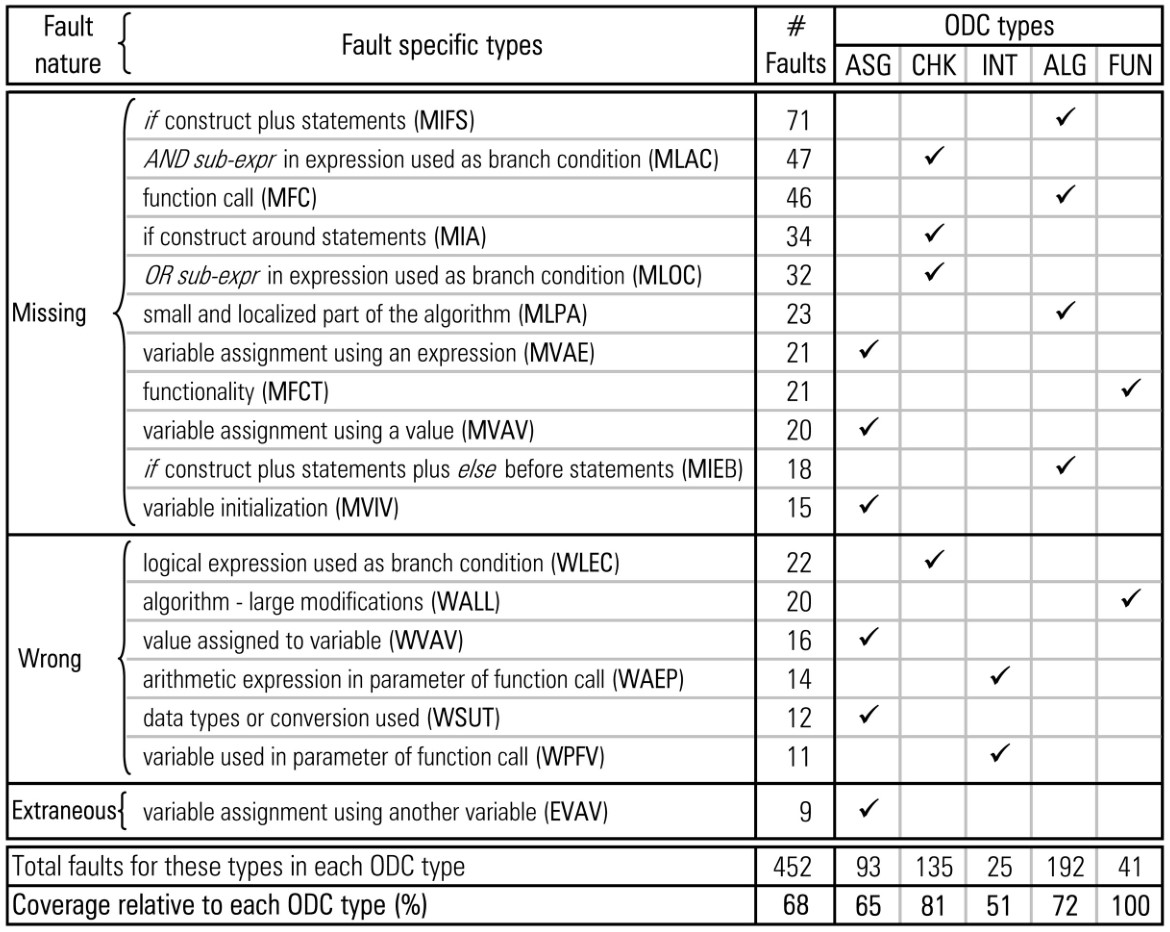
\includegraphics[width=1\textwidth]{representative_faults.jpg}
% \end{tabular}
% \caption{\small \sl \red{Fault coverage of the representative fault types.} \cite{duraes2005thesis} \label{tab:representative_faults}}
% \end{table}


%In this work
%deliberate how


% \marginnote{especificar as abreviaturas...}[0cm]
% \\textbf{acs{cots}} A \acl{cots}
% \acl{g-swfit}
% \acl{odc}

I had the opportunity to access an application that inject faults before compile time (at source code level), named SAFE. I will describe it in next section, as well as others.

\clearpage
\subsection{Software implemented fault injection of software faults}
% \iftoggle{long}{\red{In the next subsections, I will describe some fault injectors that have been previously done.}\\}

Above, I will describe some tools that use \ac{swifi} technique and made some improvements in this area of research.

\subsubsection{JACA Tool}

JACA\cite{regina2003jaca} is a tool that has been made to validate Java applications. It injects high-level software faults and is based on computational reflection to inject interface faults in Java applications
\cite{martins2002jaca}. \\

\subsubsection{J-SWFIT}

Java Software Fault Injection Tool\cite{sanches2011j} is a tool that doesn't need the source code to perform the injection, the mutation of the code is performed directly at byte-code level.\\

\subsubsection{SAFE by Robert Natella}

Safe is an application to inject realistic software faults in programs coded in C and C++.
This tool uses MCPP as parser, to get the tree of code. The decision of using MCPP instead of GCC parser was a workaround for some of the shortcomings of the GCC's C preprocessor.

After that, are written some files, variations of original files (code with simple mutations) with the operator applied.
Robert Natella implemented thirteen operators in SAFE, same as João Durães\cite{duraes2006emulation}, but Robert implemented at source code level, and João at binary level.

The fault injector under development will be similar in terms of output, code files with changes made in it. However, its creation is justified since we don't have access to the code developed by Robert Natella and the fault injector will be more maintainable and easy to use, using Java Language and not involving the MCCP prepocessor that is already outdated.\\

% (executable only) of Robert Natella, named SAFE, that injects software faults, as I also intended to do ().

\clearpage
\subsection{ODC Model}
\acl{odc}\cite{bridge1998orthogonal} Model is a framework developed by IBM\cite{chillarege2004orthogonal}, created to improve the level of technology available to assist the decisions of a software engineer, by measurement and analysis.
ODC can be used to classify and analyze defects during software development.

%\cite{lyu1996handbook}
For that, this model has eight categories:

\begin{itemize}
	\item \textbf{Function} - This defect affects significant capability, end-user features, product \acl{api}, interface with hardware architecture, or global structure(s). It would require a formal design change.
	\item \textbf{Assignment} - Typically, an assignment defect indicates an initialization of control blocks or a data structure.
	\item \textbf{Interface} - Problems in the interaction with other components, modules, device drivers, call statements, control blocks, or parameter lists.
	\item \textbf{Checking} - Based on the program logic that is checked and failed to validate data and values before the usage, loop conditions, etc.
	\item \textbf{Timing/serialization} - Errors that happen in shared and real-time resources.
	\item \textbf{Build/package/merge} - Errors that occur in the integration of library systems, management of changes, or in version control.
	\item \textbf{Documentation} - Errors in the documentation can be propagated to publications and maintenance notes.
	\item \textbf{Algorithm} - Problems that can be fixed by re-implementing an algorithm or local data structure, include efficiency or correctness that affects the task.
\end{itemize}

This model was used by João Durães, in his field-study, as a starting point for fault classification.

\clearpage
\subsection{CRASH Scale}
% \subsection{Analyze the effects}

\iftoggle{long}{\red{The fault injected results are equal to the real software faults?}}


After the compilation and execution of the programs, the results need to be evaluated. To measure that, I will use the \textit{Koopman's CRASH Scale}\cite{koopman1997comparing}:

\begin{itemize}
	\item \textbf{C}atastrophic - Operating System crashed or multiple tasks affected;
	\item \textbf{R}estart - Task or process hangs, requiring restart;
	\item \textbf{A}bort - Task or process aborts abnormally (i.e. ``code dump'' or ``segmentation violation'');
	\item \textbf{S}ilent - Test Process exits without an error code returned when one should exist;
	\item \textbf{H}indering - Test Process exits with an error code not relevant to the situation or incorrect error code returned;
	\item \textbf{P}ass - The module exits properly, possibly with an appropriate error code.
\end{itemize}

The order of the letters in the word CRASH represents the impact to the operating system (Catastrophic is the worse and Hindering the least severe).

This \textit{CRASH Scale} is a way to group the results of the effect of faults on an end-use system, mainly from the operating system perspective, by the severity.

\iftoggle{long}{\orange{Esta parte é particularmente importante: a classificação dos efeitos. Creio que há mais a dizer, pois fará parte do plano futuro de desenvolvimento classificar o que cada programa defeituoso faz.}}

\clearpage
\section{Research objectives and approach method}

In this section are discussed the main aspects in study.

\subsection{Cloud Computing}



To understand a little more what the Cloud Computing means:\\

\textit{``Cloud computing is a model for enabling ubiquitous, convenient, on-demand network access to a shared pool of configurable computing resources (e.g., networks, servers, storage, applications, and services) that can be rapidly provisioned and released with minimal management effort or service provider interaction.''}\cite{mell2011nist}.\\

Cloud Computing is a new way to delivery IT services on-demand (utility-oriented and Internet-centric). These services include all the computational power: from hardware infrastructure as a set of virtual machines to software services as development platforms and distributed applications.

\begin{figure}[!ht]
\begin{center}
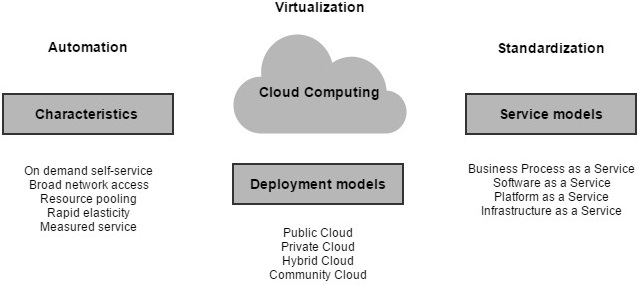
\includegraphics[width=0.9\textwidth]{cloudcomputing.jpg}
\caption{\small \sl Cloud computing overview.\label{fig:cloudcomputing}}
\end{center}
\end{figure}

Below, it will be described in relation to characteristics, deployment models and service models\cite{schouten2013ibm}.

The characteristics of Cloud Computing are:
\begin{itemize}
	\item \textbf{On demand self-service} 	- The users can request and manage their cloud computing resources without requiring human interaction, over a web-based self-service portal.
	\item \textbf{Broad network access 	}	- Provide access over the network and using standard way through by several costumers (e.g., mobile phones, tablets, laptops and workstations).
	\item \textbf{Resource pooling 		}	- The computer resources are pooled to serve multiple customers through the safe separation of the resources at logical level.
	\item \textbf{Rapid elasticity 		}	- Capability of resources to be elastically provisioned and released. Making sure that the application will have exactly the capacity that it needs at any point of time.
	\item \textbf{Measured service 		}	- The service is monitored, measured, and reported transparently based on the usage. The costumers pay in accordance with the service spent.
\end{itemize}

Four models of deployment:
\begin{itemize}
	%and treat effectively a lot of requests.}
	\item \textbf{Private Cloud}   - It is a single-tenant cloud solution utilizing client hardware and software, is located inside the client firewall or even data center. The sensitive information is maintained inside of organization. It has the disadvantage of not having ability to scale on demand.

	\item \textbf{Community Cloud} - It is shared by organizations with similar interests, supported by a specific community, sharing the same mission, security requirements, etc.

	\item \textbf{Public Cloud}    - It is available to the public or to a group of a big company. It is a multi-tenant cloud solution owned by cloud service provider, which delivers shared hardware and software to costumer private network (mostly the Internet) and data centers.

	\item \textbf{Hybrid Cloud}    - Composed by two or more services (private, community or public), together by standard technologies or proprietary that allows portability. Takes advantages from the best of private and public. Example: A client can implement a private cloud for applications with sensitive data and a public cloud for other data, non-sensitive.
\end{itemize}

Four levels of Cloud Computing Service Models:

\begin{itemize}
	\item \textbf{\acl{iaas}} - As the name suggests, provides a computing infrastructure, such as virtual machines, firewalls, load balancers, IP addresses, virtual local area networks and others. Examples: \textit{Amazon EC2}, \textit{Windows Azure}.

	\item \textbf{\acl{paas}} - Provides a computing platform that normally includes operating system, programming language execution environment, database, web server and others. Examples: \textit{AWS Elastic Beanstalk}, \textit{Windows Azure}, \textit{Heroku}.

	\item \textbf{\acl{saas}} - Provides access to application software often referred as \textit{on-demand self-service} software. Use it without install, setup or run the application.
	% Service provider does all those things for you.
	Examples: \textit{Google Apps}, \textit{Microsoft Office 365}.

	\item \textbf{\acl{bpaas}} - This model supply an entire horizontal or vertical business process and builds on top of any of services previously described.

\end{itemize}

In the figure \ref{fig:cloudcomputingservicemodels}, is possible to verify the differences between the different models.

\begin{figure}[!ht]
\begin{center}
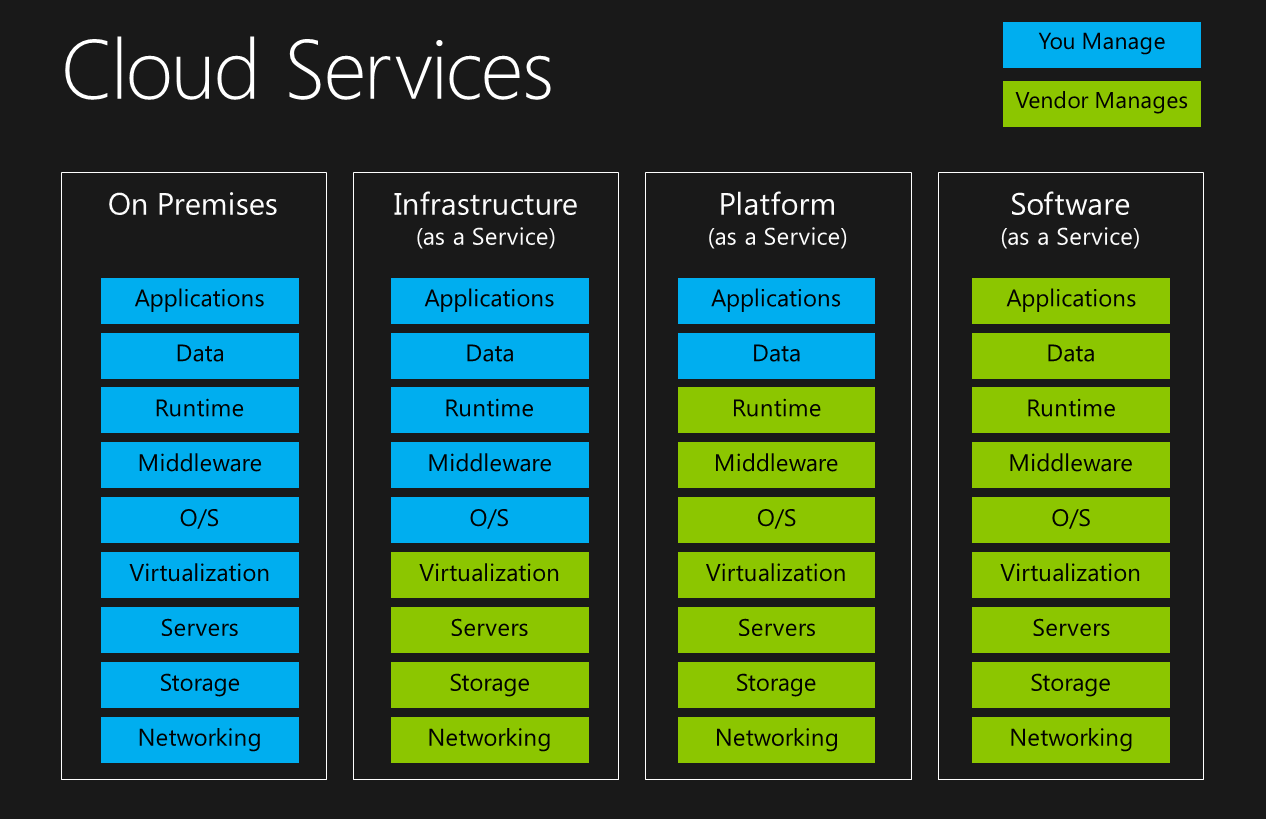
\includegraphics[width=1\textwidth]{cloud-computing-service-models2.png}
\caption{\small \sl Cloud computing service models. \textit{Source: www.hanusoftware.com/}\label{fig:cloudcomputingservicemodels}}
\end{center}
\end{figure}

Nevertheless, such as any computer system, cloud computing isn't free of external disturbances\cite{wolter2012resilience}, the most important are:
\begin{itemize}
 	\item \textbf{Security attacks - } any try to gain unauthorized access;
 	\item \textbf{Accidents - } an unplanned incident, resulting in damage;
 	\item \textbf{Power surges - } an interruption of the flow of electricity;
 	% \item \textbf{Workload faults - } cenas;
 	\item \textbf{Malfunction - } bugs cause function wrongly, or not function at all;
 	\item \textbf{Worms - } malware computer program;
 	\item \textbf{\acl{ddos} attacks - } a try to make an network resource unavailable.
 \end{itemize}

\clearpage
\subsection{Tools}
 % - GCC Parser, Bison and Eclipse CDT}

In the beginning of planning the basic software without any user interface, it was necessary to research the best applications, as the best way for using them to obtain panned results (fault injector).

For that, I thought that can be used the same tools that I used in Compilers course, Lex and Yacc or use others like Eclipse CDT, GCC Parser or MCPP preprocessor.\\

%\red{For parsing the code, analyze and modify it,}

\subsubsection{Bison/Yacc}

Yacc is a parser generator and Bison is a GNU version of Yacc. What yacc does is takes the tokens and build a tree from it to check the syntax of the program. The tokens are built by the lexer and they are declared in yacc specification file. To use this tool would be necessary to define the tokens and the grammar of the C language which would be laborious and time consuming, that is not the focus of this internship.

\subsubsection{Eclipse CDT}

Eclipse CDT, as the name suggests, is a plugin for Eclipse that give a fully functional C and C++ Integrated Development Environment.
Some of the features included in this plugin that are interesting for this project:
\begin{itemize}
	\item Source navigation;
	\item Code editor with syntax highlighting;
	\item Source code refactoring and code generation.
\end{itemize}

It's possible to use this plugin in standalone mode, importing .jar files to the project.
Using it, I can code Fault Injector in Java, making the software more maintainable and easy to use, write, compile and debug.
\\

\subsubsection{GCC Parser}

Nowadays, GCC use a hand-written parser to improve syntactic error diagnostics, giving people meaningful messages on syntax errors. Nevertheless, to use this parser in the injector, the learning curve would be very high and it would take a long time, since it is very optimized.\\

\subsubsection{MCPP}

MCPP is a portable C and C++ preprocessor with many features related with validation. Robert Natella used it as workaround for some of shortcomings of the GCC's C preprocessor. Now, it is outdated, the last update was at 28-05-2013.\\

% Finally, I decided to use
In the end, I chose to use the Eclipse CDT Plugin as standalone (only importing libraries to project), because of my abilities in programming in Java Language, the maintainability of software developed in it and the low learning level that the developers need to modify it.\\

\clearpage
\section{Fault injector development}

The Fault Injector currently in development is coded in Java using Eclipse CDT Plugin, and it will have thirteen operators (can be seen in Table \ref{tab:faultEmulationOperators})\cite{duraes2005thesis}. Furthermore, the fault injector can have two schema's of trigger the faults: spatial and temporal. In the temporal way, the insertion of the fault is given by the time associate with the execution in system. Whereas, in the spatial way, the fault is injected when reaches the specified zone where the particular operator can be applied.

\begin{table}[!ht]
\begin{tabular}{|l|p{12cm}|}
\hline
\textbf{Fault Type}		& \multicolumn{1}{c|}{\textbf{Description}}		\\ \hline \hline
\acs{mfc}        				& \Acl{mfc}  									\\ \hline
\acs{mia}        				& \Acl{mia}  									\\ \hline
\acs{mieb}       				& \Acl{mieb} 									\\ \hline
\acs{mifs}       				& \Acl{mifs} 									\\ \hline
\acs{mlac}       				& \Acl{mlac} 									\\ \hline
\acs{mloc}       				& \Acl{mloc} 									\\ \hline
\acs{mlpa}       				& \Acl{mlpa} 									\\ \hline
\acs{mvae}       				& \Acl{mvae} 									\\ \hline
\acs{mvav}       				& \Acl{mvav} 									\\ \hline
\acs{mviv}       				& \Acl{mviv} 									\\ \hline
\acs{waep}       				& \Acl{waep} 									\\ \hline
\acs{wpfv}       				& \Acl{wpfv} 									\\ \hline
\acs{wvav}       				& \Acl{wvav} 									\\ \hline
\end{tabular}
\caption{\small \sl Fault emulation operators.\label{tab:faultEmulationOperators}}
\end{table}

In the beginning of this project, I considered all the eighteen operators more representative in the open source software. However, after collecting information and analyze them, I verify that I don't have all the necessary information to implement all the eighteen operators due to various reasons.
The operators that will not be implemented can be seen in the table \ref{tab:otherfaultEmulationOperators}.

\begin{table}[!ht]
\begin{tabular}{|l|p{12cm}|}
\hline
\textbf{Fault Type}		& \multicolumn{1}{c|}{\textbf{Description}}		\\ \hline \hline
\acs{evav}        				& \Acl{evav}  									\\ \hline
\acs{mfct}        				& \Acl{mfct}  									\\ \hline
\acs{wall}       				& \Acl{wall} 									\\ \hline
\acs{wlec}       				& \Acl{wlec} 									\\ \hline
\acs{wsut}       				& \Acl{wsut} 									\\ \hline
\end{tabular}
\caption{\small \sl Other fault emulation operators.\label{tab:otherfaultEmulationOperators}}
\end{table}

The reasons for which they not be implemented are:

\begin{itemize}
	\item Production of a large number of mutations;
	\item Definition of the operators inconclusive;
	% \item Unfeasible implementation;
	\item Little or no information about the cases where it is applied;
	\item Can produce warnings or even errors while compile;
	\item Low representation in relation to the other operators (can be seen in field study of João Durães).
\end{itemize}

To overtake some of these reasons, it was necessary to obtain the data with which João Durães performed the field-study, or do a new field-study. However, due to the time limit, it would be unfeasible at this time.

% \iftoggle{long}{\orange{Convém explicar e contextualizar tudo isto. Nas notas ao longo do semestre creio que há muitos argumentos que fomos colecionando.}}

\clearpage
\subsection{Generate derivations}

I chose to use a set of the most representative faults, previously specified by João Durães\cite{duraes2006emulation} according to his data-field results, specified individually further down:

	\subsubsection{\textbf{\acs{mfc}}} - \Acl{mfc}

	The emulation of this operator is based in the remotion of a function call in a context where the returned value is not used. Nevertheless, to do the remotion, the constraints below need to be validated.
	\begin{itemize}
		\item \textbf{\acs{c01}} - \Acl{c01};
		\item \textbf{\acs{c02}} - \Acl{c02}.
	\end{itemize}

	\subsubsection{\textbf{\acs{mia}}} - \Acl{mia} - \green{\textbf{Implemented}}

	This operator simulates a missing \textit{if} condition surrounding a set of statements. This causes that the statements are always executed and not only when the condition of \textit{if} is true.
	\begin{itemize}
		\item \textbf{\acs{c08}} - \Acl{c08};
		\item \textbf{\acs{c09}} - \Acl{c09}.
	\end{itemize}

	\subsubsection{\textbf{\acs{mieb}}} - \Acl{mieb} - \green{\textbf{Implemented}}

	This operator generates derivations of the source code of applications by removing the if construct plus statements plus else before statements. To apply this operator I need to verify the constraint above:
	\begin{itemize}
		\item \textbf{\acs{c08n}} - \Acl{c08n}.
	\end{itemize}

	This constraint doesn't exists in João Durães specification, but as this operator cannot be applied in all situations, I specified and implemented it.

	\subsubsection{\textbf{\acs{mifs}}} - \Acl{mifs} - \green{\textbf{Implemented}}

	The application of this operator changes the source code with the remotion of one \textit{if} construct and the statements surrounded by it.
	But, to do that, I need to verify the constraints above:
	\begin{itemize}
		\item \textbf{\acs{c02}} - \Acl{c02};
		\item \textbf{\acs{c08}} - \Acl{c08};
		\item \textbf{\acs{c09}} - \Acl{c09}.
	\end{itemize}

	\subsubsection{\textbf{\acs{mlac}}} - \Acl{mlac} - \green{\textbf{Implemented}}

	This operator emulates the remotion of part of a logical expression used in a branch condition. To apply this operator, the code must have at least two branch conditions linked together with the logical operator AND. With an AND operator, if one of the sub-expressions is \textit{false} all the expression will be \textit{false} and the condition will fail.
	\begin{itemize}
		\item \textbf{\acs{c12}} - \Acl{c12}.
	\end{itemize}

	\subsubsection{\textbf{\acs{mloc}}} - \Acl{mloc} - \green{\textbf{Implemented}}

	This operator emulates the remotion of part of a logical expression used in a branch condition. To apply this operator, the code must have at least two branch conditions linked together with the logical operator OR. It is only necessary that one of the sub-expressions be true to the entire expression are evaluated as true. This operator has only one constraint:

	\begin{itemize}
		\item \textbf{\acs{c12}} - \Acl{c12}.
	\end{itemize}

	\subsubsection{\textbf{\acs{mlpa}}} - \Acl{mlpa}

	As the name suggests, this operator emulates the omission of a small and localized part of the algorithm.

	\begin{itemize}
		\item \textbf{\acs{c02}} - \Acl{c02};
		\item \textbf{\acs{c10}} - \Acl{c10}.
	\end{itemize}

	The constraint \textbf{\ac{c02}} guarantees that don't be removed all the statements in a block, because this would not correspond to a realistic fault. This type of faults never involved the remotion of \textit{if} or \textit{if-else} and loop constructs (the omitted statements were always function calls and assignments) guaranteed by constraint \textbf{\ac{c10}}.

	\subsubsection{\textbf{\acs{mvae}}} - \Acl{mvae}

	This operator reproduces the omission of a given local variable with an expression. However, not when is the first assignment to a variable, an initialization, guaranteed by the constraint \textbf{\acs{c07}}.

	\begin{itemize}
		\item \textbf{\acs{c02}} - \Acl{c02};
		\item \textbf{\acs{c03}} - \Acl{c03};
		\item \textbf{\acs{c06}} - \Acl{c06};
		\item \textbf{\acs{c07}} - \Acl{c07}.
	\end{itemize}

	\subsubsection{\textbf{\acs{mvav}}} - \Acl{mvav}

	Operator \textbf{\ac{mvav}} is similar to operator \textbf{\ac{mvae}}, with the difference that it emulates the remotion of the assignment of a given local variable with a constant value instead of an expression. The constraints related with this operator are the same of \textbf{\ac{mvae}}:

	\begin{itemize}
		\item \textbf{\acs{c02}} - \Acl{c02};
		\item \textbf{\acs{c03}} - \Acl{c03};
		\item \textbf{\acs{c06}} - \Acl{c06};
		\item \textbf{\acs{c07}} - \Acl{c07}.
	\end{itemize}

	\subsubsection{\textbf{\acs{mviv}}} - \Acl{mviv}

	As the name suggests, this operator represents the remotion of a given local variable initialization with a constant value. The fact that this operator only searches for variable initialization induce that only the first occurrence of an assignment to a particular variable are readable to apply this type of fault, this is guaranteed by the constraint \textbf{\acs{c04}}. The constraint \textbf{\acs{c05}} verifies if the assignment doesn't occur inside a loop, because one assignment of this type occurs several times. Nevertheless, this operator has other associated constraints:

	\begin{itemize}
		\item \textbf{\acs{c02}} - \Acl{c02};
		\item \textbf{\acs{c03}} - \Acl{c03};
		\item \textbf{\acs{c04}} - \Acl{c04};
		\item \textbf{\acs{c05}} - \Acl{c05};
		\item \textbf{\acs{c06}} - \Acl{c06}.
	\end{itemize}


%	\hypertarget{wlec}{}
%	\subsubsection{\textbf{\acs{wlec}}} - \Acl{wlec}
%	\hypertarget{wall}{}
%	\subsubsection{\textbf{\acs{wall}}} - \Acl{wall}


	\subsubsection{\textbf{\acs{waep}}} - \Acl{waep}

	This operator represents the modification of the expression used as parameter of a function call.

%	\hypertarget{wsut}{}
%	\subsubsection{\textbf{\acs{wsut}}} - \Acl{wsut}

	\subsubsection{\textbf{\acs{wpfv}}} - \Acl{wpfv}

	Operator \ac{wpfv}, as the name suggests, modify the variables used as parameter in a function call, given a wrong variable. The use of constraint \textbf{\acs{c11}} guarantee that there must be at least two variable in the module.

	\begin{itemize}
		\item \textbf{\acs{c03}} - \Acl{c03};
		\item \textbf{\acs{c11}} - \Acl{c11}.
	\end{itemize}

	\subsubsection{\textbf{\acs{wvav}}} - \Acl{wvav}

	As the name suggests, this operator simulate an assignment of a wrong value to a variable. This value is obtained by the inversion of bits of the least significant byte of the early value. To do that, the operator needs to verify the following constraints:

	\begin{itemize}
		\item \textbf{\acs{c03}} - \Acl{c03};
		\item \textbf{\acs{c04}} - \Acl{c04};
		\item \textbf{\acs{c06}} - \Acl{c06}.
	\end{itemize}

The above operators may change, since they were specified for implementation at the binary level and in this project will be implemented at the source code level.
After applying the operators in the code of tree, will be generated modified files to use in the testing process.

%\subsubsection{Fault Types - Extraneous}
%\begin{itemize}
%	\item \textbf{EVAV} - variable assignment using another variable
%\end{itemize}
\clearpage
\subsection{Constraints}

As was discussed in the specification of the operators, the operators cannot be applied in all the situations and need to complying with the specification in accordance with the field-data study, which has been done by João Durães. To do that, the operators need to verify the constraints below.

\begin{table}[!ht]
\centering
\begin{tabular}{|c|p{12cm}|}
\hline
\textbf{Constraints}            & \multicolumn{1}{c|}{\textbf{Description}}                                     \\ \hline \hline
\textbf{C01}         			& \Acl{c01} \\ \hline
\textbf{C02}         			& \Acl{c02} \\ \hline
\textbf{C03}         			& \Acl{c03} \\ \hline
\textbf{C04}         			& \Acl{c04} \\ \hline
\textbf{C05}         			& \Acl{c05} \\ \hline
\textbf{C06}         			& \Acl{c06} \\ \hline
\textbf{C07}         			& \Acl{c07} \\ \hline
\textbf{C08}         			& \Acl{c08} \\ \hline
\textbf{C09}         			& \Acl{c09} \\ \hline
\textbf{C10}         			& \Acl{c10} \\ \hline
\textbf{C11}         			& \Acl{c11} \\ \hline
\end{tabular}
\caption{\small \sl Fault emulation contraints defined by João Durães.\label{tab:faultEmulationConstraintsDuraes}}
\end{table}

The constraint \textbf{C07} is similar to constraint \textbf{C04}, one is the negation of another. This happens too with the constraint \textbf{C08} and \textbf{C08n}.
Constraint \textbf{c10} is the same as constraint \textbf{C09}, but with one additional restriction: the statements need to be contiguous and need to belong to the same code block.

When was implementing the operators \textbf{\ac{mieb}} and \textbf{\ac{mloc}}, it was necessary to define the constraints \textbf{\ac{c08n}} and \textbf{\ac{c12}}. The constraint \textbf{\ac{c08n}} was created because of the operator \textbf{\ac{mieb}} cannot be applied to an \textit{if} without an \textit{else} construct and the constraint \textbf{\ac{c12}} was created because the operator \textbf{\ac{mloc}} can't be emulated in a branch with only one condition.

\begin{table}[!ht]
\centering
\begin{tabular}{|c|p{12cm}|}
\hline
\textbf{Constraints}            & \multicolumn{1}{c|}{\textbf{Description}}                                     \\ \hline \hline
\textbf{C08n}         & \Acl{c08n} \\ \hline
\textbf{C12}         & \Acl{c12} \\ \hline
\end{tabular}
\caption{\small \sl Other constraints.\label{tab:otherConstraints}}
\end{table}

These constraints can be modified during the implementation of the other operators that aren't implemented yet.

\clearpage
\section{Work and implications}

In the figure \ref{fig:decisions}, can be seen an overview of the main decisions that I did during this semester.

Since the beginning of this project, it was expected that I should create a fault injector. However, as stated earlier, in the beginning it was to inject faults in hardware but due to the postponement of six months, and the development of the project related to inject faults in hardware, the project was modified to inject faults in software.

After take that decision, I had to choose the technique that would use injection faults, from three: at binary code level in the execution environment, at object code level in the compilation or before the compilation at source code. I selected source code level because there are made some tools, which inject faults in execution environment, p.e. by João Durães. Previously, Robert Natella had coded a tool from this type, using MCPP as C preprocessor at his thesis of PhD.
All these reasons would lead to inject faults at object code level in the compilation, but the use of this technique in the development of fault injector and the evaluation of the robustness of the cloud would be a great effort and too much work for a master's thesis. Hence, it was decided to inject fault before the compilation, at the source code of applications. The use of this technique provides the emulation of realistic software faults done by real programmers.

Despite already exists Robert's tool to inject faults at source code, the injector under development will use the capabilities of Java, such as the maintainability and the easy to use, to inject faults in source code coded in C language.

The faults will be injected in C code because of the extensive knowledge of the supervisors and because of the work already done by João Durães at PhD, in the specification of the operators, be based on a field-study of open source software coded in that language.

Then, I evaluated the software possibilities to parse the code and get the AST tree. I chose to use the Eclipse CDT Plugin mainly because of my abilities in programming in Java Language, but also by the features that it has, such as source navigation, source code refactoring and code generation.

In spite of the Eclipse CDT has many attractive characteristics for this project, the implementation of the first operator was not easy. After some time to understand the tool and the structure of classes through Javadoc, it was even necessary to obtain more information from those who know and really work with it, by accessing the list: cdt-dev@eclipse.org.

After exchanging some emails with Thomas Corbat, I learned that the Eclipse CDT doesn't allow the creation of a new tree of code by making changes in the original tree. Moreover, I had two options, use reflection to get the modifications from ASTWriter and pass it to ASTRewrite to get the code with the changes done or get the source code of CDT and change it to avoid the use of reflection.

Initially, I opted to use reflection, despite knowing that it's not a neat solution and is generally slower than equivalent native code, but after understand better the flow of Eclipse CDT, I get the source and change it to avoid the use of reflection.

After that, I finally had the first operator implemented, using recursion. However, I can traverse the tree without using recursion, using the Visitor Pattern, making the code simpler, cleaner and safer. Then I modified all the recursion to the visitor pattern.


 % as standalone (only importing libraries to project), because of my abilities in programming in Java Language, the maintainability of software developed in it and the low learning levelthat the developers need to modify it


 \iftoggle{long}{\red{Built three separated modules:
\begin{itemize}
	\item Generate the derivations of main code of selected programs;
	\item Verify and analyze the effect of produced faults;
	\item Compile the programs with injected faults, by using make file.
\end{itemize}}}

% \iftoggle{long}{\red{Problems with the rewriting of tree}}
% \iftoggle{long}{\red{Reflection}}
% \iftoggle{long}{\red{But I was forced to take decisions after that, for example, after creating the tree of code, I can go through the tree in the recursive way or using \textit{Visitor Pattern}.}}

\begin{figure}[!ht]
\begin{center}
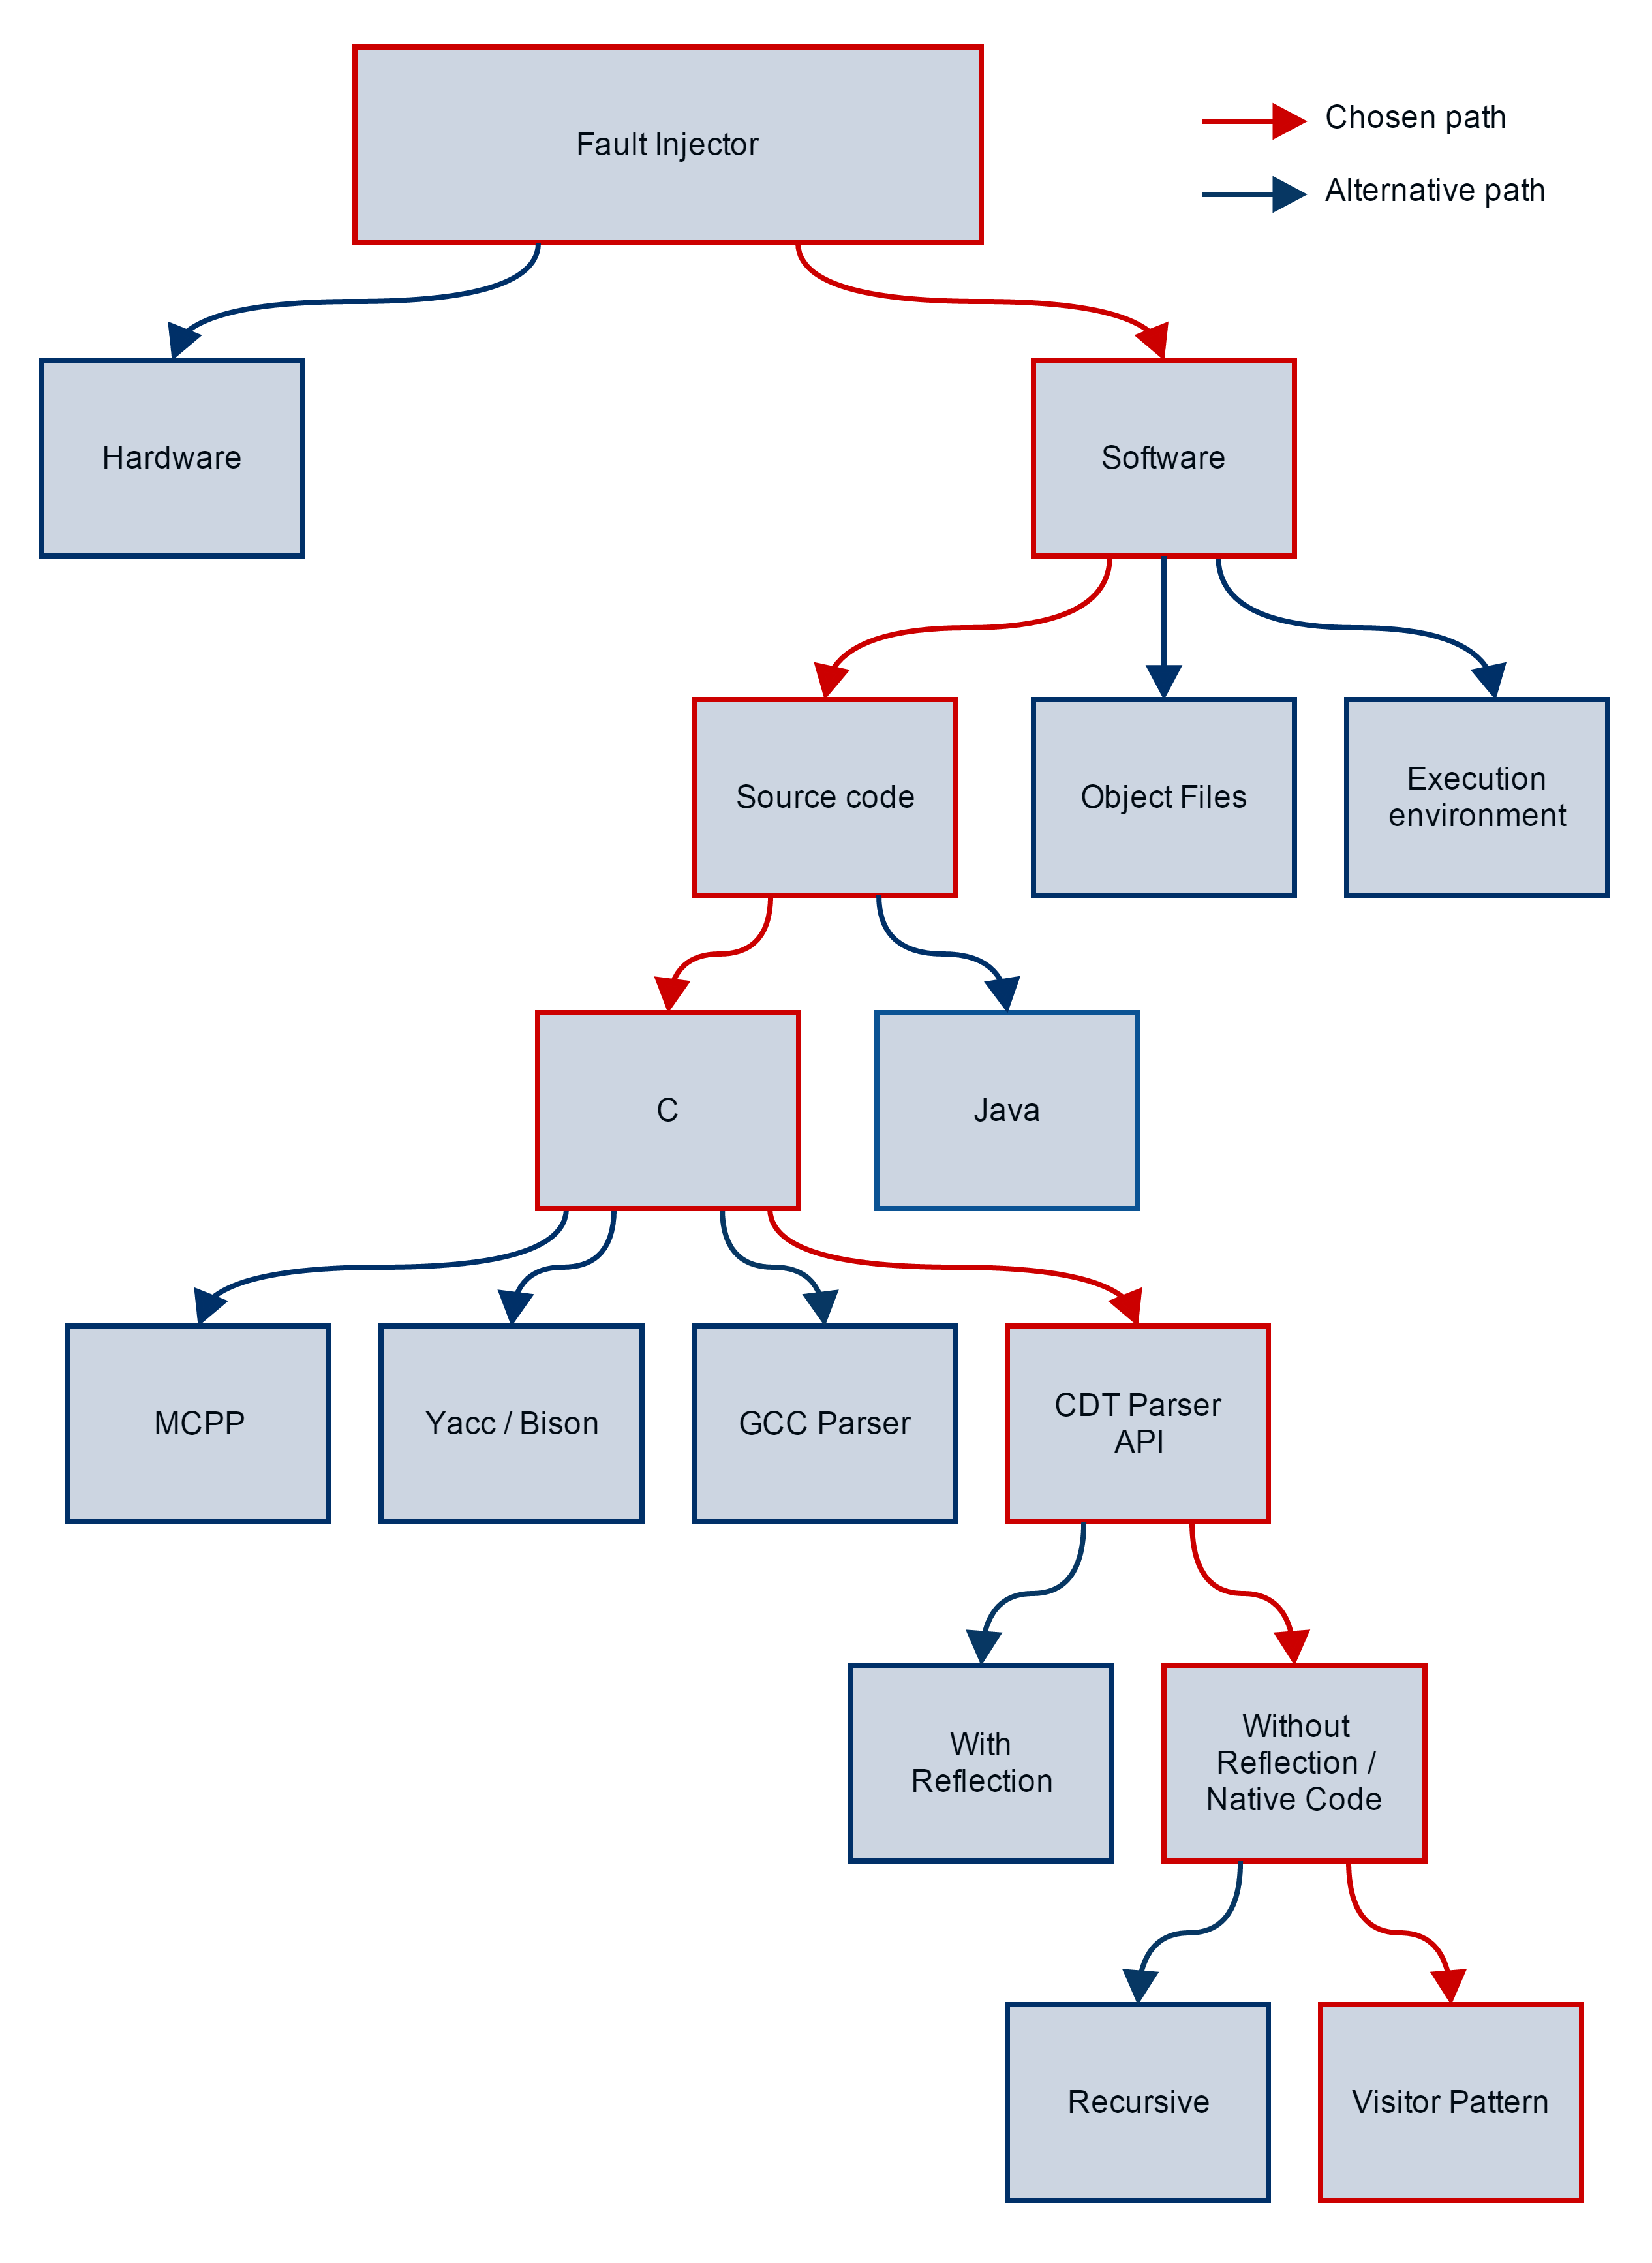
\includegraphics[width=0.8\textwidth]{decisions.png}
\caption{\small \sl Decision tree.\label{fig:decisions}}
\end{center}
\end{figure}

\clearpage

The figure \ref{fig:mockup}, represents an overview of the fault injection tool. Initially, the fault injector starts by read the source code of a file coded in C, it is analyzed and is created a AST tree. To inject a fault, the fault injector finds the node where it can be injected, and modify it, according to operator specification. After this, the AST tree is rewritten, getting the code again, now with modifications. Finally, with the comparison of the two codes, source code and source code with mutations, it is made a \textit{diff}, so obtaining a summary of the changes made between files.

\begin{figure}[!ht]
\begin{center}
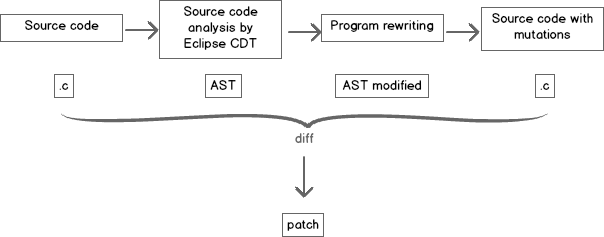
\includegraphics[width=1\textwidth]{mockup.png}
\caption{\small \sl Overview of the injection tool.\label{fig:mockup}}
\end{center}
\end{figure}

% \iftoggle{long}{\red{Justificar a utilização de patchs}}
I chose to use the \textit{diff} tool, since the use of this tool allows the creation of smaller files with only the changes that are made, instead of using all the code with the modifications made in it.
